\chapter{Review of Related Literature}
\label{sec:rrl} 

\section{dPCR Droplet Classification Methods}
\label{sec:dpcrclassifiers}

\subsection{Threshold}
\label{sec:threshold}
The most common method in classifying positive and negative droplets are by enforcing a hard threshold. All droplets with a fluorescence amplitude greater than this threshold is then classified as positive, and negative otherwise. The following sections explore how a threshold can be determined with statistical methods.

One popular tool incorporated with automatic thresholding is the QuantaSoft software. The QuantaSoft software is the dPCR analysis tool that comes with the Bio-Rad droplet digital PCR System package. It allows for the setting up of sample and experiments, running and controlling the instrument, and the analysis of the NA concentration \cite{BioRad2019}. According to the Bio-Rad Laboratories website (https://www.bio-rad.com), it has been a leading product developer for over 65 years in the research fields of life science and clinical diagnostics. Among its popular focus areas, dPCR is one of its most featured technology, providing droplet dPCR instruments; kits, reagents and assays; and other consumables. Several studies in hospitals \cite{Lopez2016,Chen2018,Abed2017,Tagliapietra2020}, public health \cite{Hussain2017,Nystrand2018}, food safety \cite{Chen2020,Capobianco2020,Basanisi2020}, upto environmental quality \cite{Hamaguchi2018,Jahne2020,Dobnik2016,Mauvisseau2019} have found the Bio-Rad QuantaSoft dPCR systems useful for their analyses. 

Of all the features of the QuantaSoft software, the focus of this section is on how the software sets the threshold. By default, QuantaSoft sets an automatic threshold to the single-well or multiple-well amplitude data; a demonstration is shown in \figref{fig:demoQuantThreshold}. As with other automated tools, its documentation recommends reviewing this threshold to make changes if needed; and thus, manually setting the threshold is also allowed. Unfortunately, the calculation of the automatic threshold is not publicly available.

\begin{figure}[h]
    \centering
    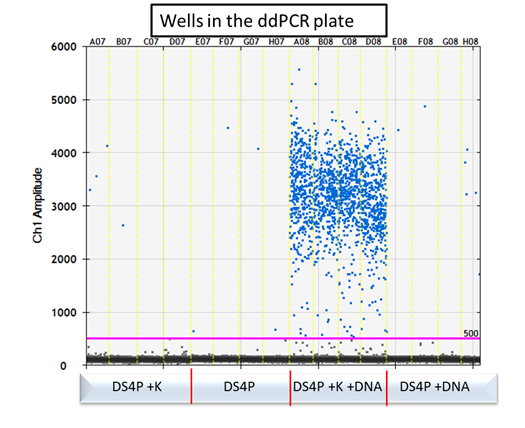
\includegraphics[max size={\textwidth}{\textheight}]{quantasoftThreshold.png}
    \caption[QuantaSoft threshold from a study]{QuantaSoft threshold in pink line from \cite{hussainThreshold}}
        \label{fig:demoQuantThreshold}
\end{figure}


%  What type of experiments are suitable for Quantasoft?
TODO - look for Quantasoft experiments

%  What are the results of experiments using Quantasoft?

[1]
For samples exhibiting a substantial amount of intermediate fluorescence, the QuantaSoft software fails to determine a threshold, resulting in a "No call" output. This was the case when a study of two bacteria \cite{Dreo2014} was ran on very high concentration. In the case of low bacteria concentrations, droplets near the negative droplets were classified as positives. 

TODO - look for 2 more other Quantasoft experiments with bad results
% [2]

% [3]

%  What are their recommendations of using the Quantasoft software?
These studies concluded that the QuantaSoft software requires a well-optimized assay with good discrimination of positive and negative droplets for its threshold to be reliable.


\subsection{Population Detection of Gaussian Kernel Densities}
\label{sec:peakdetectionkde}
Although not named in the paper of \citeA{Lievens2016}, cloudy is the name of the function in their source code provided in their supplementary file. Cloudy implements the following steps for threshold calculation, which is also documented in their paper:
\begin{enumerate}
    \item Estimate the density function of the fluorescence using a Guassian kernel density with a minimum bandwith of 50
    \item Identify density peaks using a sliding window approach. The subsequent steps will differ according to if one, two, or more than three peaks were found.  But generally, the proceeding steps are followed.
    \item For each population found through the peaks, its location and spread is initially estimated using the median \(\hat{\mu}\) and \(\hat{\sigma}\). Assuming normality, the latter is estimated as half the peak width at 60-65\% of its maximum height.
    \item Refine the estimates using a reiterative method, first initialized with \(a=4\).
    \item Re-estimate \(\hat{\mu}\) and \(\hat{\sigma}\) using only the observations within \(\hat{\mu} \pm (a \cdot \hat{\sigma})\).
    \item Recalculate \(a=4.55 + 0.35 \cdot log(k) + 0.045 \cdot log(k)^2\); where \(k\) is the kurtosis of the distribution
    \item Repeat steps 5-6 until stabilization.
    \item After stabilizing the estimates for all the population, the last step is different when either including or excluding rain in the final categorization. 
    \begin{enumerate}
        \item If rain is included as a category, observations within \(\hat{\mu} \pm (a \cdot \hat{\sigma})\) are then classified as members of that population; observations not falling within any population are classified as rain.
        \item If rain categorization is not of interest, then a threshold \(\theta=\hat{\mu_n} + 1.5 \cdot a_n + \hat{\sigma_n}\) is calculated; where \(n\) is a population.  
    \end{enumerate}

\end{enumerate}

In summary, the cloudy algorithm uses the Gaussian kernel density and normality assumptions to detect peaks, which are then considered as populations. From then population density parameters are estimated based on specified formulas. A range or a single threshold is then calculated for classifying droplets as positive, negative, or optionally, rain.

Special cases such as overlapping population boundaries and threshold placement problems are also checked in their source code. It is worth noting that in step 6, the formula for re-calculating \(a\) for density parameter estimation is based on the analysis of their in-house data, and should be used with caution when implementing for other unobserved NA targets. The rain classification rule in step 8(a) also poses a problem for fluorescence densities that are heavily skewed. \figref{fig:skeweddist} left panel reveals the distribution of negative droplets to be heavily skewed to the right, thereby causing their exclusion to be labeled as negative due to the symmetry of the categorization rule (right panel).

\begin{figure}[h]
    \centering
    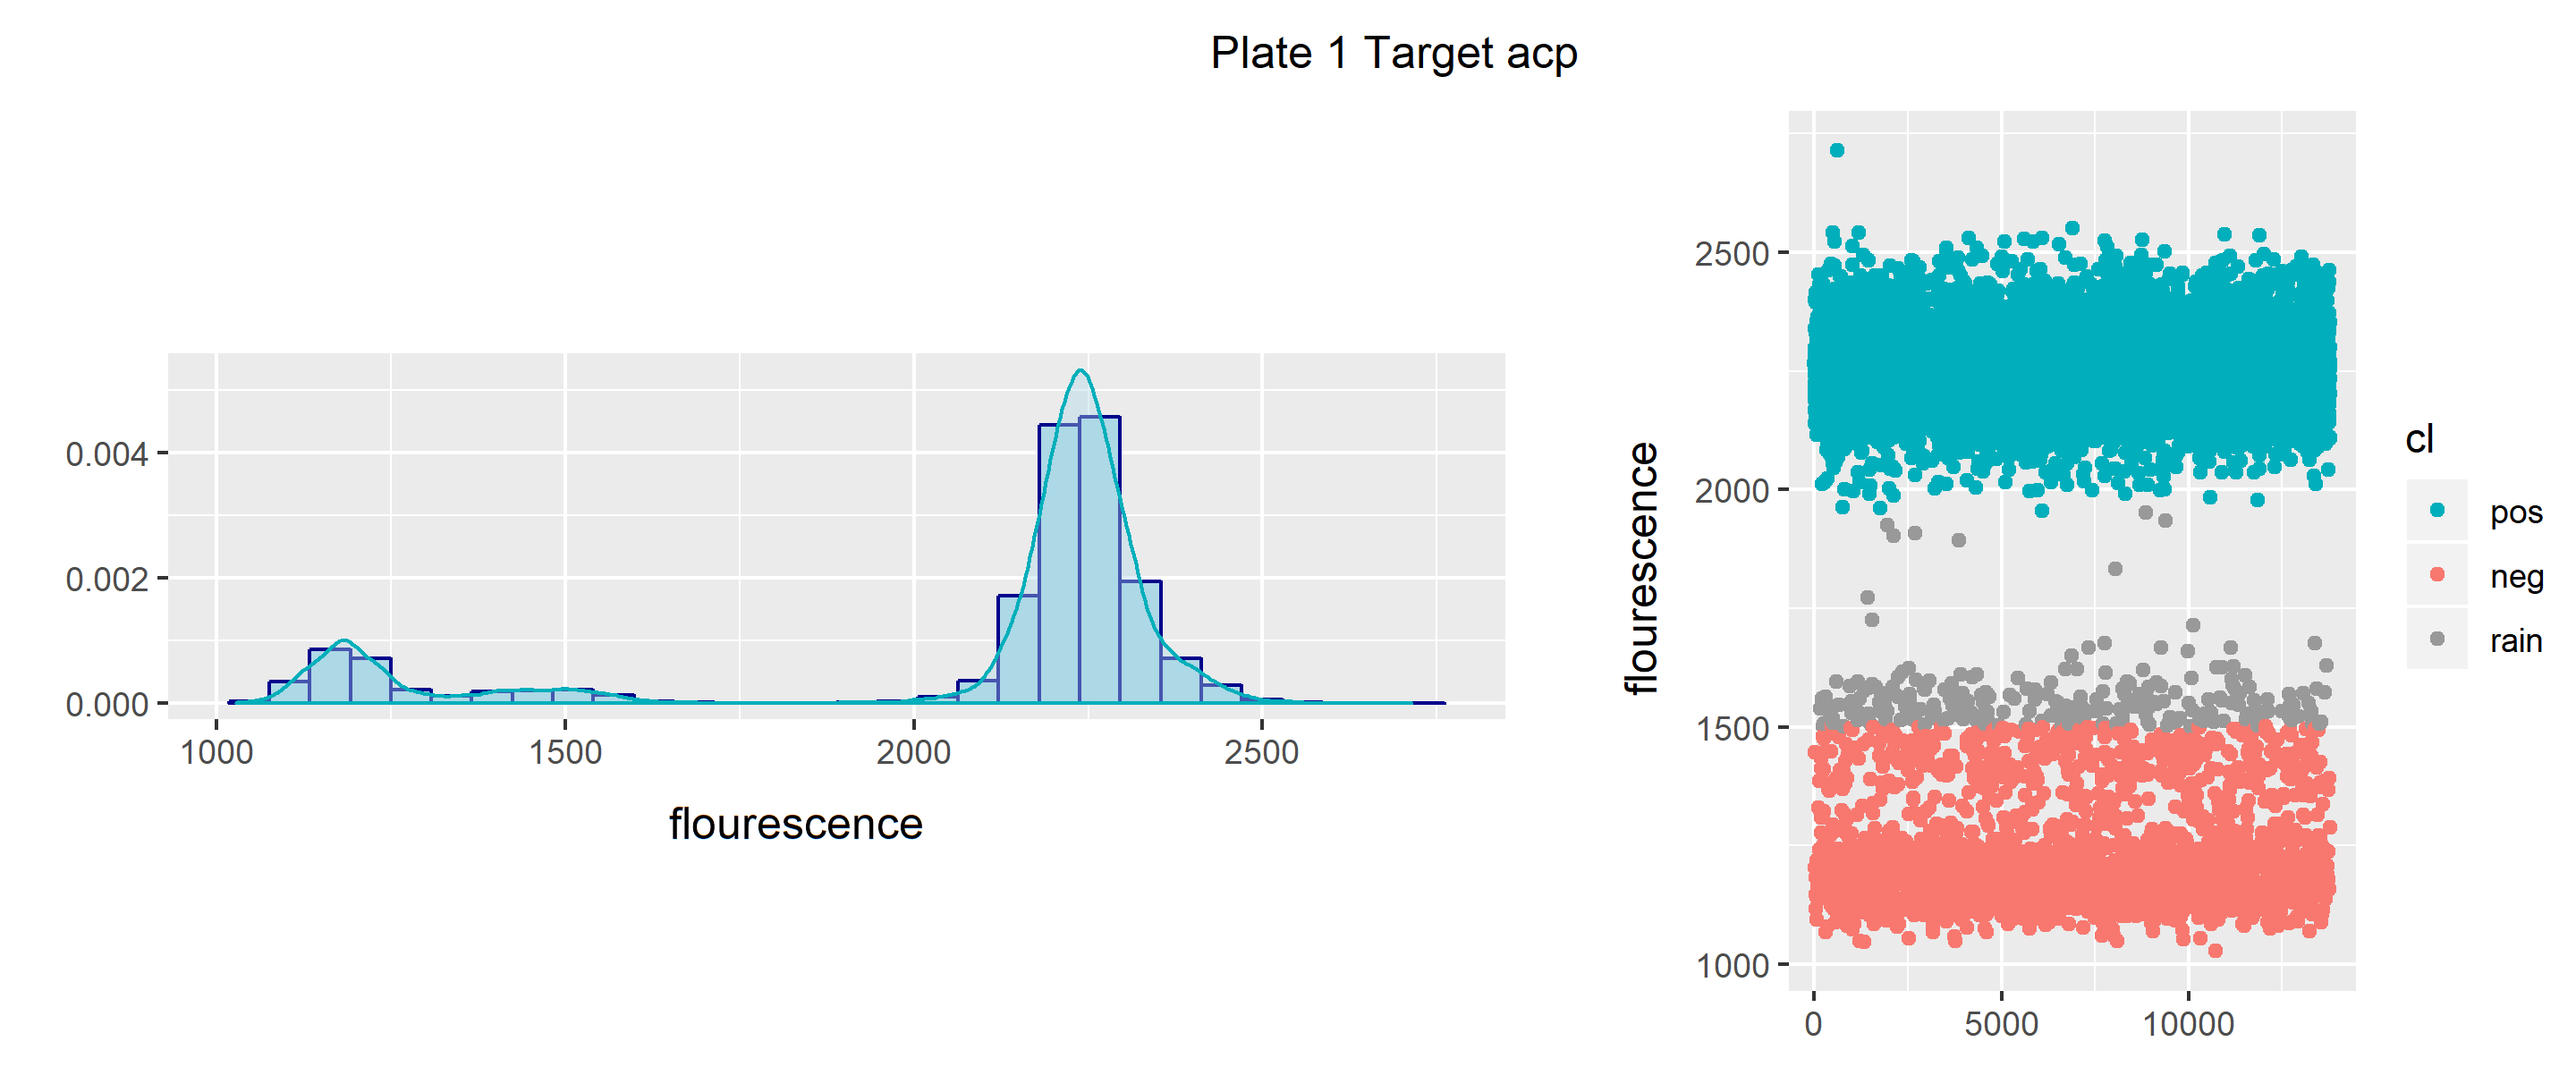
\includegraphics[max size={\textwidth}{\textheight}]{skeweddist.png}
    \caption[Fluorescence distribution of DNA target acp]{One replicate of the DNA target acp Plate 1 from \citeA{Lievens2016} dataset. Left panel shows the fluorescence densities. Right panel is the result of droplet categorization using cloudy}
        \label{fig:skeweddist}
\end{figure}

TODO - add their results from this algorithm

\subsection{K Nearest Neighbors}
\label{sec:knn}
% TODO - Define definetherain and its benefits


definetherain follows these steps for classification:
\begin{itemize}
    \item Setup a control well of known input copy numbers. 
    \item Cluster using k-nearest neighbor with \(k=2\). 
    \item Using cluster means and standard deviation, rain in subsequent test samples are classified if it is not within the range of mean \(\pm\) 3 standard deviations of the negative cluster and mean \(\pm\) 3 standard deviations of the positive cluster.
\end{itemize}

\begin{figure}[h]
    \centering
    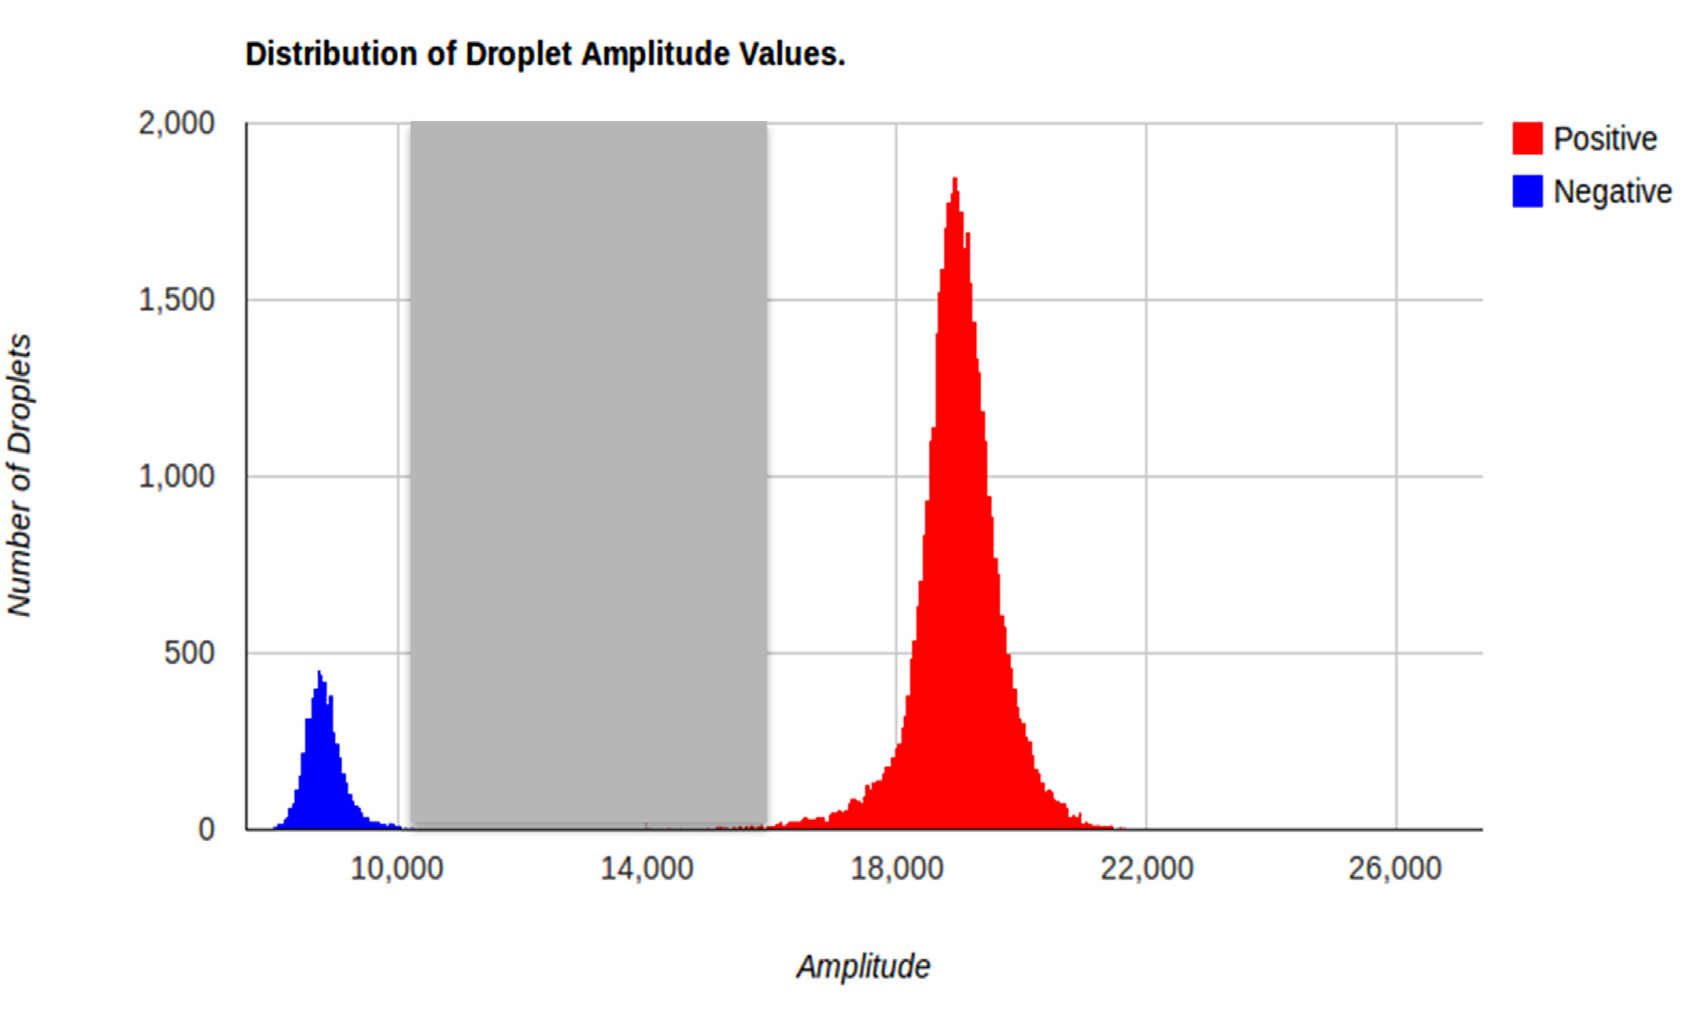
\includegraphics[max size={\textwidth}{\textheight}]{dtrsample.png}
    \caption[Determined thresholds calculated by definetherain]{Determined thresholds calculated by definetherain, reprinted from \cite{jonesThreshold}}
        \label{fig:dtrsample}
\end{figure}

% TODO - Studies that use dtr


\subsection{Non-parametric Mixture Models}
\label{sec:nonparametricmixmodels}

\section{Model-Based Clustering}
\label{sec:modelbasedclustering}

